\documentclass[journal,hidelinks]{IEEEtran}
\usepackage[utf8]{inputenc}
\usepackage[
  pdftitle={Assignment \#3},
  pdfauthor={Andrei Purcarus},
  pdfsubject={ECSE-526 -- Artificial Intelligence}
]{hyperref}
\usepackage{graphicx}
\usepackage[all]{hypcap}
\usepackage{cleveref}
\usepackage{indentfirst}
\usepackage[per-mode=symbol]{siunitx}

\title{ECSE-526 \\ Artificial Intelligence \\ Assignment \#3}
\author{Andrei~Purcarus,~260631911,~\IEEEmembership{McGill~University}}

\begin{document}
\sloppy

\maketitle

\begin{abstract}

An reinforcement learning agent was designed to learn to play the Atari 2600 game of Q*bert on the Arcade Learning Environment platform using the Q-learning algorithm. This was achieved by extracting the game's features from the ALE screen and RAM and encoding them into a localized state representation for which utilities could be learned. The result was a strong game playing agent that could achieve an average score of 38,800 when factoring in a 25\% chance of its actions being ignored by the ALE.

\end{abstract}

\section{Introduction}

\IEEEPARstart{T}{his} report describes the creation of an agent that uses reinforcement learning to learn to play the Atari 2600 game of Q*bert using the Arcade Learning Environment (ALE) \cite{bellemare_2013_arcade}. First, we describe how we extracted the necessary game features from the ALE. Then, we describe how we encoded those features into a compact state representation in order to provide generalization. Then, we describe our approach to exploration. Finally, we evaluate the performance of our agent using multiple ALE random seeds. In order to avoid having to learn a transition model for the states in the game, which would be difficult given the stochastic nature of the ALE and the presence of multiple enemies, we used the Q-learning algorithm to learn an effective game playing policy by assigning utilities to (state, action) pairs.

\section{ALE}

First, we had to extract several game features from the ALE. The game of Q*bert has $7$ possible entities that appear on the pyramid (Q*bert, Red Ball, Purple Ball, Coily, Flying Discs, Sam, Green Ball), and $3$ possible colors of blocks for each level (Start, Intermediate, Destination) \cite{greg_chance_atari_1997}. To obtain these features, we used screen captures of the game to define fixed rectangles on the screen where features could be located. Then, we extracted the color present in each rectangle and used it to determine the value of a feature. Using this approach, we were able to determine the block colors and the locations of Q*bert and the other entities. We were also able to extract the Destination color for a given level by looking at the color of the score display, as well as the Start color from the initial block colors at the beginning of a level.

One problem with this approach was that Coily sometimes jumps to the top of the pyramid and is not rendered by the game. In addition, if two enemies are located on the same horizontal row, they are rendered on alternate frames, which could lead to Coily not being detected by the agent. To resolve these problems, we used the game RAM to obtain Coily's position and correct the results of the image extraction.

Finally, we also used the game RAM to trigger state updates. We found that the game accepts an action from the player when the first byte in RAM is $0$ and the last bit in RAM is $1$. This allowed us to time our updates properly to state transitions and assign rewards to our agent appropriately. In addition, we found out that the ALE has an option to randomly ignore player input enabled by default. For training purposes, we disabled this option.

\section{Generalization}

Next, we had to encode the features extracted from the ALE into a manageable and generalized state space. Our first step towards generalization was to encode each block color into one of three possible types (Start, Intermediate, Destination). This massively reduces the state space by converting each block from $128$ possible colors to $3$ possible types. In addition, it generalizes the behavior learned across levels, since the agent will be able to learn to treat different color combinations as the same depending on the Start and Destination colors of the given level.

Our next step was to combine different enemies together into the same entity. For example, Sam and the green ball were both labeled as green enemies, and the red and purple balls were both labeled as dangerous balls. This further reduces the state space and allows for similar responses to states that contain similar enemies.

Finally, we approached generalization by taking a localized view of the pyramid from Q*bert's perspective. Thus, we only looked at the blocks and enemies that were next to Q*bert at any given time, and ignored anything else on the board. This is equivalent to a "distance metric" where two states are considered the same if they have the same local properties. We tried four different approaches to this, which we describe next.

\subsection{Monolithic}

Our first approach was to use a monolithic state encoding, in which a single learner learns both how to deal with the block colors and how to deal with enemies. To achieve this, we encoded Q*bert's block type, the types of the $4$ neighboring blocks, the locations of any dangerous enemies at a distance of $2$ or less from Q*bert, the locations of any green enemies at a distance of $1$ from Q*bert, and the locations of any discs at a distance of $2$ or less from Q*bert. In addition, we assigned to the "blocks" under discs the same block type as the block at the top of the pyramid, given that that is where it would end up if it jumps on the disc. Note that here we have lumped together Coily with the dangerous balls described above in order to keep the state space as small as possible.

Our choice of distances is motivated by the fact that dangerous enemies can still pose a threat at a distance of $2$ away, since Coily might jump towards Q*bert while Q*bert is jumping towards Coily, resulting in death. This was not as much of a concern for green enemies, since these cannot damage Q*bert. However, this approach has two major drawbacks. The first is that the joint presence of block types and enemies in the state description means that the agent fails to learn that jumping towards a dangerous enemy is always bad until it sees the results of jumping towards an enemy for all possible block type combinations. The second is that the localized view of the block types means that it lacks a global view of where to go after it clears the blocks surrounding it. Adding such a global view would further compound the first drawback by increasing the size of the state space. We address both of these issues with our subsequent architectures.

\subsection{Subsumption-V1}

To deal with the drawbacks of the previous architecture, we used a subsumption architecture \cite{brooks_robust_1986} to split the state space between two independent learners. One learner, the Block Solver, focuses on learning to solve the block puzzles, while the other, the Enemy Avoider, focuses on learning to avoid dangerous enemies while getting points from green enemies. The Enemy Avoider was made to suppress the Block Solver whenever a dangerous enemy was present at a distance of $2$ or less from Q*bert, or a green enemy was present at a distance of $1$ or less from Q*bert. In order to assign split rewards to learners, we used the fact that block color changes award rewards of $25$ points while all other rewards are multiples of $100$ \cite{greg_chance_atari_1997}. Thus, we assigned the reward modulo $100$ to the Block Solver and the rest to the Enemy Avoider.

To encode the state for the Block Solver, we used a similar local encoding as for the monolithic learner, with the types of the blocks at a distance of $1$ or less encoded, as well as replacing discs by the top block of the pyramid. However, to solve the locality problem, we also encoded, for each of the $4$ directions, a binary variable indicating if there are any blocks in that direction with a given type. This allows the learner to see beyond its immediate surroundings while keeping the state space small. In addition, we encoded the current level divided by $4$ in order to allow the agent to learn different behaviors for different level rules, since the rules change every $4$ levels.

To encode the state for the Enemy Avoider, we used the same encoding of enemies as in the monolithic learner. We then added a measure of the current Q*bert position. This allows it to learn different policies depending on Q*bert's location in the pyramid. For example, if it keeps dying after getting stuck in the corner, it should learn that running away towards the corner leads to entrapment and should thus be avoided.

This architecture allows for the generalization of enemy avoidance across arbitrary block states. In addition, it has the effect of reducing our state space substantially, allowing for faster learning. Also, since the rewards are split, both agents can learn even if one is suppressing the other. This effectively doubles the learning rate of the subsumption-v1 agent.

\subsection{Subsumption-V2}

We next experimented with potential improvements over the subsumption-v1 agent. Since our Enemy Avoider state space was quite small, we tried splitting the encoding of Coily from the encodings of the other dangerous enemies. This allows the agent to learn different policies for dealing with Coily and the purple ball, which makes sense since Coily follows Q*bert while the purple ball just falls down the pyramid.

\subsection{Subsumption-V3}

Finally, we also tried a similar architecture to subsumption-v2, but with Coily's location being encoded whenever it was at a distance of $3$ or less from Q*bert. The Enemy Avoider was also modified to suppress the Block Solver whenever Coily was at a distance of $3$ or less from Q*bert. This change is mostly motivated by the fact that we noticed that Coily sometimes jumps ahead by $2$ blocks instead of $1$, which has the effect of killing off an unsuspecting Q*bert using subsumption-v2. By enlarging the agent's line of sight, we hoped to avoid this situation. However, increasing the distance for Coily also limits the agent's block solving ability, since it will be stuck in enemy avoidance for a larger fraction of the time.

\subsection{Comparison}

A comparison of these four agents is shown in \Cref{fig:generalization}. All agents used the exploration policy of threshold $10$, which is described in the next section. This figure clearly shows that all the subsumption models outclassed the monolithic model and were able to learn much faster. This was expected since the monolithic learner needs to learn how to avoid enemies for every possible combination of block types before it stops dying. It fails to generalize that jumping towards Coily has the same result for all possible block states, and thus is slower to learn. The subsumption architecture solves this by making enemy avoidance independent of surrounding block types.

\begin{figure}[!htb]
  \centering
  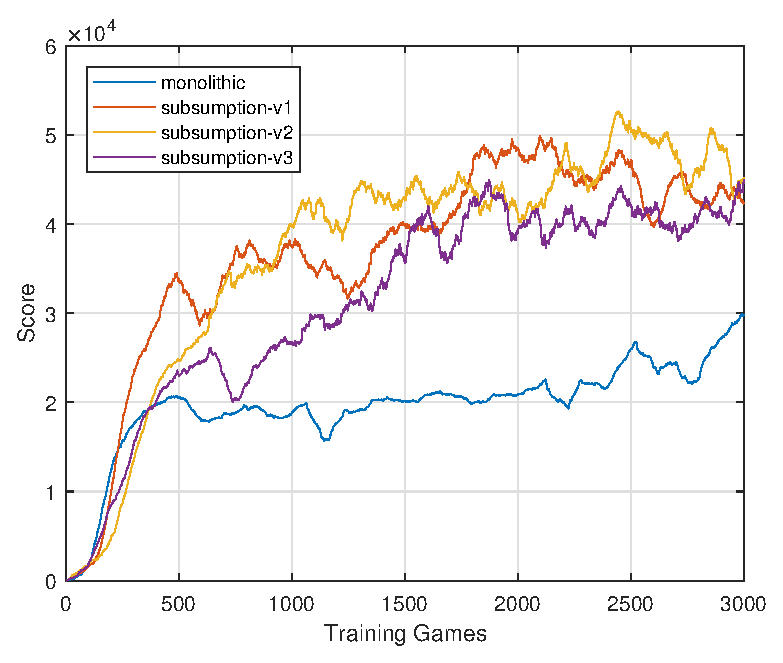
\includegraphics[width=0.8\columnwidth]{figures/generalization.eps}
  \caption{Scores achieved during training for the four agent models with an exploration policy of threshold $10$. The results were passed through a $100$-point moving average filter for smoothing.}
  \label{fig:generalization}
\end{figure}

In addition, we can see that the subsumption-v1 model, being smaller in state space, learns faster at the beginning. However, all three subsumption architectures converge to similar results after $3000$ training games. The reason for this could be that after clearing level 8, the blocks start reverting back to their Start color if hit while in the Destination color. A policy to solve such levels would require a global view of the pyramid, which is something we don't have. Thus, the score from that point onwards is a function of how long the agent can stay alive, since flipping blocks will keep giving points indefinitely. The results thus show that after only $3000$ games, all three agents are roughly equally good at staying alive.

\section{Exploration}

In order to allow our agents to explore the state space, we tried several different approaches. In order to maintain a consistent implementation across all our exploration policies, we did not explicitly use an optimistic prior on the (state, action) utilities. Instead, we kept track of the number of times each (state, action) pair was visited. Each time an action had to be selected, we computed the minimum number of times any action in the current state had been visited, which we called $N$. Then, we selected a random action if $f(N)$ returned true, and a greedy action if $f(N)$ returned false, where $f$ is an exploration policy. The following sections detail three possible choices for $f$.

\subsection{Epsilon\_Greedy}

Our simplest choice of exploration policy is the epsilon\_greedy policy. This policy ignores $N$ and simply returns true with probability $\epsilon$ and false with probability $1-\epsilon$. This function is simple to implement, but it results in a non-decaying randomness over time, which severely limits the agent's performance after it learns a good policy.

\subsection{Inverse\_Proportional}

Our second choice of policy is the inverse\_proportional policy, which returns true with probability $1/(N+1)$ and false with probability $N/(N+1)$. This approach gradually reduces the randomness as we explore the state space, and thus will produce better performance in the long run as the agent stops trying random actions after it learns a good policy.

\subsection{Threshold}

Our final choice of policy is the threshold policy, which simply returns true if $N$ is less than some threshold value $N_{min}$ and false otherwise. This policy will keep suggesting random actions until all actions have been tried at least $N_{min}$ times. However, since the choice of action is random and is not biased towards unexplored actions, it will take roughly $4$ times longer to stop choosing random actions than if we focused on trying the actions least tried so far. However, implementing that behavior would require a different interface, and hence we chose this approach instead.

\subsection{Comparison}

A comparison of these three exploration policies is shown in \Cref{fig:exploration}, for which we used $\epsilon = 0.05$ and $N_{min} = 10$ with the subsumption-v2 learner. This figure clearly shows that the epsilon\_greedy policy learns faster at first, which was expected since it has a fixed randomness of $0.05$ while the other two start at close to $1.0$. We can also see that the inverse\_proportional policy catches up relatively quickly and has a similar performance to the epsilon\_greedy policy after $1000$ games, which was again expected since its randomness drops quickly at first and slows down as it tries actions multiple times. Finally, we notice that while the threshold policy starts off slowly, it starts performing really well after it has reached its threshold for enough actions. This happens because it stops choosing random actions completely after a certain number of tries for each action, which results in less accidental deaths. This policy is limited, however, in that it stops exploring relatively quickly, which means the other two learners might overcome it in the long run.

\begin{figure}[!htb]
  \centering
  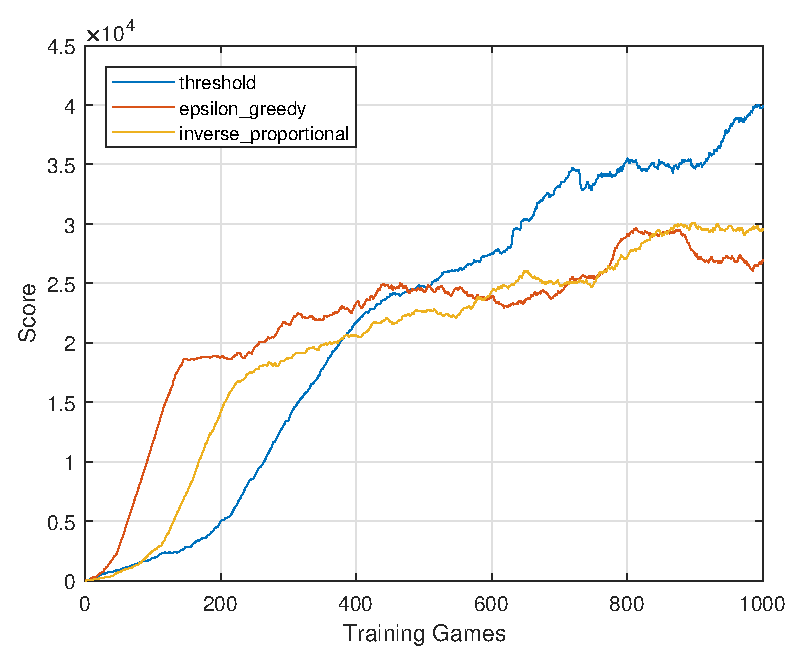
\includegraphics[width=0.8\columnwidth]{figures/exploration.eps}
  \caption{Scores achieved during training for a subsumption-v2 learner using three different exploration policies. We used $\epsilon = 0.05$ and $N_{min} = 10$. The results were passed through a $100$-point moving average filter for smoothing.}
  \label{fig:exploration}
\end{figure}

\section{Performance}

We analyzed the performance of the agents during the learning process in previous sections, with the results shown in \Cref{fig:generalization,fig:exploration}. These figures clearly show that the agents can improve their performance through reinforcement learning. We now look at how well this learning generalizes across different seeds and with different random events.

To achieve this, we first trained the subsumption-v2 agent with a threshold $10$ exploration policy for $10,000$ games and the seed $123$. Then, we turned on the ALE option to randomly ignore player input in order to increase the stochasticity of the trials. We next measured the agent's performance over $10$ games each for a random selection of $5$ seeds. The average results are shown in \Cref{tab:perf}. We can see from this table that the utility values learned for the $123$ seed generalize well for other seeds, with a strong average performance of around $38,800$ points.

\begin{table}[!htb]
	\centering
	\caption{Performance results for the subsumption-v2 agent with a threshold $10$ exploration policy after $10,000$ training games. The scores were averaged over $10$ games with the given seeds.}
	\label{tab:perf}
	\resizebox{0.8\columnwidth}{!}{\begin{tabular}{|l|l|l|l|l|l|}
    \hline
		\textbf{Seed} & 6236 & 318534 & 475133 & 482403 & 984110 \\ \hline
    \textbf{Score} & 42798 & 39668 & 37783 & 36830 & 36870 \\ \hline
	\end{tabular}}
\end{table}

During observation of game play, we noticed that the performance of the agent was mostly dictated by the quality of its enemy avoidance. For levels 1-8, the blocks do not revert back to their Start colors after being hit in their Destination colors, and so the agent must learn to hit all the blocks to progress. However, once the agent reaches level 9, the blocks do revert, and the agent has great difficulty in learning a policy to solve the resulting block puzzle. However, since the blocks revert back to the Start color, the level provides an essentially infinite supply of rewards as long as the agent can stay alive. Therefore, once the agent has learned to get to level 9, survival is the primary factor in accumulating points. With the subsumption architecture, this behavior was very well learned, resulting in point totals upwards of $100,000$ on some games. During our observations, the agent could even sometimes reach level 11, as shown in \Cref{fig:level-11}, though it did so randomly and could not learn a policy to do so consistently. We also noticed that with the ALE random action option enabled, the chance of dying increased and the results in \Cref{tab:perf} only show an average of $38,800$ points. This is most likely due to the fact that enemy avoidance requires precise timing, and the ALE ignoring an action to move away from Coily could easily result in death.

\begin{figure}[!htb]
  \centering
  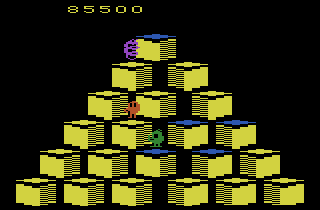
\includegraphics[width=0.8\columnwidth]{images/level-11.png}
  \caption{The subsumption-v2 agent with a threshold $10$ exploration policy reaching level 11.}
  \label{fig:level-11}
\end{figure}

\section{Conclusions}

In conclusion, we created an agent that uses reinforcement learning to learn to play the Atari 2600 game of Q*bert. Using a subsumption architecture and localized state encoding, we were able to achieve scores upwards of $100,000$, with an average score over multiple seeds of $38,800$ when using a $\SI{25}{\percent}$ probability of actions being ignored by the ALE.

Several improvements could be made to achieve better results. First, the use of a function approximation to the state encoding would allow for better generalization by reducing the hypothesis space significantly. Both linear function approximations and non-linear approximations such as neural networks could offer significant improvements, assuming the right features are selected. Second, the use of an optimistic prior function for exploration would allow our agent to learn faster. Finally, focusing the exploration on unexplored actions rather than selecting random actions until we've explored all of them would also significantly reduce learning time.

\section{Acknowledgements}

High-level strategy and ALE feature extraction were discussed with Andrew Lowther, Sean Stappas, and Juliette Valenchon.

\bibliographystyle{IEEEtran}
\bibliography{IEEEabrv,references}

\end{document}
